% -----------------------------------------------
% Template for ISMIR Papers
% 2019 version, based on previous ISMIR templates

% Requirements :
% * 6+n page length maximum
% * 4MB maximum file size
% * Copyright note must appear in the bottom left corner of first page
% * Clearer statement about citing own work in anonymized submission
% (see conference website for additional details)
% -----------------------------------------------

\documentclass{article}
\usepackage[T1]{fontenc} % add special characters (e.g., umlaute)
\usepackage[utf8]{inputenc} % set utf-8 as default input encoding
\usepackage{ismir,amsmath,cite,url}
\usepackage{graphicx}
\usepackage{color}
\usepackage{pgfplots}

%% cleveref MUST be the last import
\usepackage{cleveref}

% Optional: To use hyperref, uncomment the following.
% \usepackage[bookmarks=false,hidelinks]{hyperref}
% Mind the bookmarks=false option; bookmarks are incompatible with ismir.sty.

% Title.
% ------
\title{Fractal dimension for music similarity and patterns in symbolic music data}

% Note: Please do NOT use \thanks or a \footnote in any of the author markup

% Single address
% To use with only one author or several with the same address
% ---------------
%\oneauthor
% {Names should be omitted for double-blind reviewing}
% {Affiliations should be omitted for double-blind reviewing}

% Two addresses
% --------------
%\twoauthors
%  {First author} {School \\ Department}
%  {Second author} {Company \\ Address}

%% To make customize author list in Creative Common license, uncomment and customize the next line
%  \def\authorname{First Author, Second Author}


% Three addresses
% --------------
\threeauthors
  {First Author} {Affiliation1 \\ {\tt author1@ismir.edu}}
  {Second Author} {\bf Retain these fake authors in\\\bf submission to preserve the formatting}
  {Third Author} {Affiliation3 \\ {\tt author3@ismir.edu}}

%% To make customize author list in Creative Common license, uncomment and customize the next line
%  \def\authorname{First Author, Second Author, Third Author}

% Four or more addresses
% OR alternative format for large number of co-authors
% ------------
%\multauthor
%{First author$^1$ \hspace{1cm} Second author$^1$ \hspace{1cm} Third author$^2$} { \bfseries{Fourth author$^3$ \hspace{1cm} Fifth author$^2$ \hspace{1cm} Sixth author$^1$}\\
%  $^1$ Department of Computer Science, University , Country\\
%$^2$ International Laboratories, City, Country\\
%$^3$  Company, Address\\
%{\tt\small CorrespondenceAuthor@ismir.edu, PossibleOtherAuthor@ismir.edu}
%}
%\def\authorname{First author, Second author, Third author, Fourth author, Fifth author, Sixth author}


\sloppy % please retain sloppy command for improved formatting

\definecolor{ao(english)}{rgb}{0.0, 0.5, 0.0}
\newcommand{\alternative}[1]{{\color{ao(english)}{#1}}}
\begin{document}

%
\maketitle
%
\begin{abstract}
  Fractals are highly regular objects with repetitions at different scales.
  \alternative{(Alternative intro sentence, for a more cross-disciplinary audience in mathematics and complex system research?:
    In mathematics, a fractal is a geometric object which exhibits regularity through self-similarity --- the whole being repeated at different scales, resulting to similar parts of itself.) }
  This has a natural counterpart in music: musical patterns repeat at different granularities of time.
  The hierarchical structures in fractals and music offer a starting point to describing and detecting these varying repetitions. 
  In this paper, we explore this connection quantitatively by examining these hierarchies at different levels and computationally measure the fractal dimension in music.
  We apply our framework to compute the time series of the fractal dimensions in monophonic symbolic corpora and synthesised data.
  For these different corpora, the distance matrices of the fractal dimensions exhibit distinct differences, showing a potential means to measure music similarity. 
  We further substantiate the novelty and usefulness of the fractal dimension by reporting its low correlations with previously-studied features.
  Using our approach, we are able to obtain patterns exhibiting certain geometric properties by thresholding on the fractal dimensions, permitting the extraction of pattern candidates with the same or similar melodic contours.

\end{abstract}

\newcommand{\victor}[1]{{\color{blue}\textbf{[victor:}\textit{#1}\textbf{]}}}

\section{Introduction}
\label{sec:intro}

  Musical patterns are easily spotted by a trained performer,
even if the pattern appears under different \emph{variations}.  These
variations include transpositions, inversions, time dilations, between
others. Amongst the favorite examples of patterns showing up under a
plethora of variations are the fugues by J.S. Bach. Take
\Cref{fig:bwv861-start}, we see two patterns showing up under
inversions and transpositions in the first two bars.

\begin{figure}
  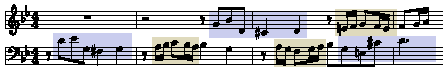
\includegraphics[width=\linewidth]{src/img/bwv861-start-section-patterns.pdf}
  \caption{Two patterns and their variations in the beginning of BWV 861}
  \label{fig:egbach}
\end{figure}

  Writting a computer program that is capable to identify these
patterns modulo their variations is no easy feat. The naive approach
would be to select a candidate pattern, then go over the whole
piece comparing interval per interval. This would have to be computed
for every possible pattern candidate. The exponential nature of this
approach makes it unrealistic and will not get us very far.

  Fractal~\cite{bouligand1928ensembles}

  In this paper we discuss an alternative, and efficient, approach to
identifying patterns in symbolic music. The idea is to assign a real
number to a potential pattern in such a way that \emph{similar}
patterns have \emph{similar} numbers. We call this the pattern
identifier.  This enables us to group patterns that differ by
$\epsilon$.  A potential pattern consists simply in a group of
notes. If we want to check whether a pattern of $n$ notes shows up but
in half tempo, for example, we can compute the pattern identifier for
all groups of contiguous $2n$ notes and compare the pattern
identifiers.

  A prime option for pattern identifier is to use 
  In this paper we propose an alternative method of mining a musical
piece for its patterns under certain variations. Instead of comparing 
the possible patterns of a musical piece for propositional equality, 
we compute a \emph{measure} that identifies the \emph{candidate pattern}.
This reduces the problem to comparing measures and deciding if they are
close enough to be considered a pattern. We use fractal dimension~\cite{fractaldimension}
as our measure. \victor{we need a better phrase or two about related
work, in the lines of: Although Fractal Geometry and Music goes a long way\cite{bigerelle2000fractal,hsu1990fractal,hsu1991self},
we are applying it to a novel part in music analisys.}

%% \textbf{Previous work} In the research area of MIR, many useful tools
%% and investigation have been made to understand the hierachical
%% structures of music.  For example, there are music musical analysis
%% assistant \cite{hamanaka2009interactive, hamanaka2005atta},
%% compositional tools \cite{hamanaka2004automatic,
%% hamanaka2005automatic}, evaluation investigation
%% \cite{mcfee2017evaluating, mcfee2015hierarchical} based on a variety
%% of hierachical structure analysis in music.  Self-similarity concepts,
%% and fractals in particular have inspired many research in audio and
%% music analysis \cite{bigerelle2000fractal,hsu1990fractal,hsu1991self}
%% and composition \cite{sukumaran2009generation,leach1995nature}.  In
%% other domain of applications, the fractal theory has been widely used
%% in investigating time series, dynamical systems, and non-linearity
%% \cite{accardo1997use, higuchi1988approach}.  To the best of our
%% knowledge, there has not been an attempt on computing the fractal
%% dimensions equivalent in symbolic music by drawing the parallel
%% between the box-counting method and hierarchical structures in music.


  Our contributions are summarized below.

\begin{itemize}
  \item We provide a novel adaptation of fractal geometry for identifying patterns
        in a musical piece under a number of variations.
  \item We have implemented our analisys as a library and made it publicly available.
  \item We have empirically shown the effectiveness of our method for musical pattern
        recognition by running our tool in a number of musical pieces.
\end{itemize}

\section{The Fractal Geometry of Symbolic Music}
\label{sec:fractal-geom}

  On this section we review the necessary parts of fractal geometry
and explain how to apply it to symbolic music notation. This enables
us to identify a pattern with a numer that is constant under
variations such as transpositions, inversions, time dilations, etc.

  The box-count (BC) dimension~\cite{find-a-ref} of a shape is a
measure of the \emph{roughness} of that shape. It coincides with the
Euclidean dimension for the familiar shapes but it is given by a Real number. 
Consequently, it is capable of capturing differences between objects with
the same eucliden dimension, for example.

\victor{dimension is invariant to a bunch of transformations, hence,
it is great for our use case}

\begin{figure}
  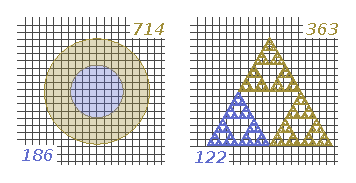
\includegraphics[width=\linewidth]{src/img/box-counting-example-alt.pdf}
  \caption{Box counting applied to a circle and the Sierpinsky Triangle. The numbers
indicate the number of boxes touched by the object before and after scaling by a factor of 2.}
  \label{fig:egboxcount}
\end{figure}

  We can approximate the box-count (BC) dimension~\cite{findref} of a
shape through a process known as box-counting. The idea is simple. We
lay a shape in a grid and count how many squares it touches, call it
$N$, then scale the shape by a factor $s$ and count how many quares it
touches again, call it $N_s$. The box-counting dimension $d$ of the
given shape is defined by the value that $\log_s(\frac{N_s}{N})$
converges to, for $s \rightarrow \infty$.  In \Cref{fig:egboxcount} we
show this technique applied to a circle and the Sierpinski
Triangle. On the left we see a small circle, touching 186 boxes, and a
circle double the size of the first, touching 714.  The circle has a
known dimension of 2. On the right we see the same for the Sierpinski
Triangle, which has a known fractal dimension of $\log_2 3 \approx 1.585$.
If we apply the BC dimension formula to the data in \Cref{fig:egboxcount} we obtain:
\[
\begin{array}{l l l l}
  d_{\circ}    &= \log_2{\frac{714}{186}} &= 1.94 &\approx 2 \\[.5em]
  d_{\tiny \triangle} &= \log_2{\frac{363}{122}} &= 1.57 &\approx 1.585 \\
\end{array}
\]

  We see that the dimension our data gives is just
\emph{approximately} the correct value. If we were to iterate this
process and plot the number of boxes touched by the scaled version of
our shapes, over the scale factor, we would see that the data for the
circle fits almost perfectly fit the curve $f(x) = cx^2$, for $c$
being a constant. The Sierpinski triangle would fit the curve $f(x) =
cx^{1.585}$.  That is, for a given shape with BC dimension $d$, the
number of boxes touched by the shape scaled by $s$ gets closer and
closer to $cs^d$ as $s$ grows.

  Note that if we rotate our Sierpinski Triangle, or translate it
to another position in the plane, or even scale it, its BC dimension
stays the same.

\subsection{Scaling in Music} 
In order to compute the BC dimension of
a potential music pattern, we must first define what to we mean by scaling 
in music. There are a variety of options for defining the meaning of
the \emph{scale factor} in symbolic music. The simplest one 
is to look at a section of music one note value at a time.
This means that at a sixteenth-note scale factor, the
line in \Cref{fig:egscalingmusic} has $xxx$ pixels, but
at the eight-note scale factor, it only has $yyy$ pixels.

\victor{finish this}

\begin{figure}
  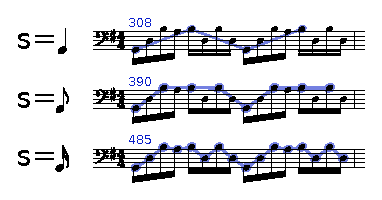
\includegraphics[width=\linewidth]{src/img/musical-scaling-example.pdf}
  \caption{The ``box-count'' under different scalings for the first measure in BWV 1007.}
  \label{fig:egscalingmusic}
\end{figure}

\subsection{Box-Count dimension of symbolic music}
\victor{write a bit about this}

\section{Experiment}

\victor{Describe the setup: wrote some haskell code,
got some data from MIDI, mined for patterns using technique shown in
\Cref{sec:fractal-geom}}

\section{Results}

\victor{What did we get out of running our tool from the midi dataset?}

\subsection{Threats to Validity}

\victor{We are not airtight. What did we not consider?}

\section{Discussion and Conclusion}

\subsection{Related and Future Work}

\subsection{Conclusion}



  

%% 
%% It is worth noting that this
%% values converges very slowly.  \victor{I'm not very attached to the plot \Cref{fig:egplots},
%% maybe use it just in case we need to fill in space?} In \Cref{fig:egplots} we see the data we
%% gathered through box counting both the circle and the Sierpinski
%% triangle plotted against the curve of their known BC dimension.
%% 
%% 
%% \begin{figure}
%% \begin{tikzpicture}
%% \begin{axis}[
%%   legend pos=north west
%% ]
%% \addplot [mark=*,blue,only marks,opacity=0.5] table {
%% 0  0
%% 1  186
%% 2  714
%% };
%% \addlegendentry{box-count Circle}
%% \addplot [mark=*,red,only marks,opacity=0.5] table {
%% 0 0
%% 1 122
%% 2 363
%% };
%% \addlegendentry{box-count Sierp.}
%% \addplot [no marks,color=black!40!blue,domain=0:3] expression {
%%   (814 / 4) * x ^ 2
%% };
%% \addlegendentry{$f(x) = c\times x^{2\textcolor{white}{.0000}}$}
%% \addplot [no marks,color=black!40!red,domain=0:3] expression {
%%   (412 / 2^1.5) * x ^ 1.5849
%% };
%% \addlegendentry{$f(x) = c\times x^{1.5849}$}
%% \end{axis}
%% \end{tikzpicture}
%% \caption{Plot of the data obtained through box counting (\Cref{fig:egboxcount})
%% versus the known dimensions of the objects.}
%% \label{fig:egplots}
%% \end{figure}



\victor{Below is the previous content}


\textbf{Storyline: hierarchical structure -> fractal dimension -> feature -> pattern discovery -> contribution }

\textbf{Hierarchical structures in music}
Music is known to have rich hierarchical structures, ranging from global forms to local phrases, from harmonic progressions to melodic patterns. 
The hierarchical structures allow us to examine music at different levels of details and time scales. For example, as shown in Figure \ref{fig:egbach}, the original piece on the top two staffs in can be summarised by the chords in the third staffs; similarly, in Figure \ref{fig:egscale}, the patterns shown on the top staff can be progressively and hierarchically reduced to the bottom staff. 
There have been many musical theories on the hierarchical structure of music, such as the General Theory of Tonal Music (GTTM) \cite{lerdahl1985generative} and the Schenkerian theory of melodic reduction \cite{forte1959schenker}.

\textbf{Hierarchies in fractal geometry}
One tool that could be used to study the hierarchical structure in music is fractal theory.
Fractal geometry is an established area of mathematics that studies self-similar patterns on different levels of details.
The concept of fractal dimension has been devised to measure the change of contents across different levels of hierarchies.
In the one-dimensional case, the fractal dimensions takes into account of the line segment lengths at different scales.
% For example, as shown in Figure \ref{fig:bc}, empirically, the fractal dimension can be measured given any contour.
Therefore, given a segment of music, one can also use the box-counting method to calculate a parallel of the fractal dimension by looking into the different levels of details exhibited on different levels of hierarchies in music.
\begin{figure}
  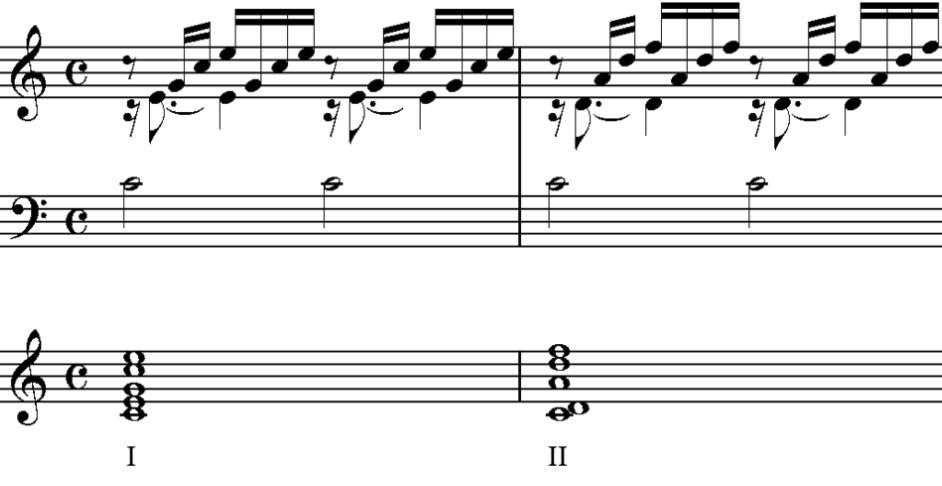
\includegraphics[width=\linewidth]{src/img/eg.png}
  \caption{Two levels of hierarchies in Bach's Preludium in C major \cite{wiki:bach}: the original piece and the underlying chords.
          The details in the first two staffs can be summarised into the chords in the third staff}
  \label{fig:egbach}
\end{figure}

\begin{figure}
  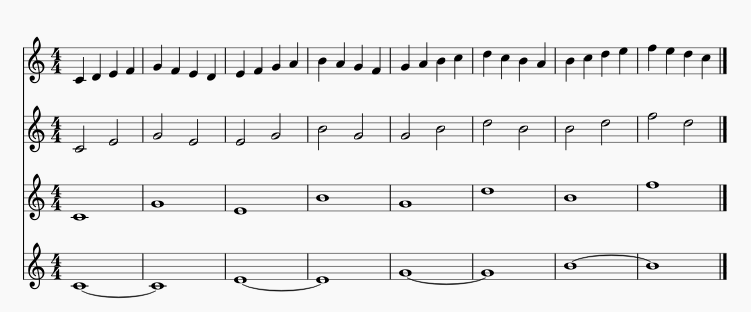
\includegraphics[width=\linewidth]{src/img/egscale.png}
  \caption{Four levels of hierarchies in an artificial example using scales: from the top to the bottom staff, we have different levels of details in different levels of hierarchies.
    The notes at different levels of hierarchies are specified based on the metrical positions of the notes.}
  \label{fig:egscale}
\end{figure}

\textbf{Contributions}
\begin{itemize}
\item  Based on fractal geometry and the hierarchical structures in music, we propose a new feature for symbolic music data.
\item  Using the proposed feature, we present a library for musical analysis and pattern discovery.
\item  We show the effectiveness of our system for musical pattern discovery and compare the proposed feature with other symbolic music features. 
\end{itemize}

\section{Methods}
Fractals are known for the property of self-similarity.
We therefore name the new feature ``similarity dimension'' in the context of MIR, and use ``fractal dimension'' in the original geometric context.

In this section, we describe how we compute the similarity dimension feature.

\subsection{Fractal dimensions and boxing counting}
Mathematically, the fractal dimension is defined as $$D=-\frac{logM}{logs}$$

where $M=Mass$, usually defined in terms of lengths or areas of the geometric objects, and $s=scaling$, usually defined as how many recursive steps has been taken in creating the fractals.

One intuition of fractal dimension is how rough or how much detail are embedded in the geometric object.
For example, the coast lines of different countries can be measured in terms of fractal dimensions by using the box-counting method \cite{sarkar1994efficient}, where one control the scaling factor $s$ and count the ``boxes'' to obtain the mass $M$.
Thus we can empirically compute fractal dimensions given any geometric objects. 

\textbf{Similarity dimension in music}
In the context of music, there have been evidences that a visual-audio correspondence exists amongst music objects \cite{thorpe2016perception}.
This can also be observed from the sheet music.
Without musical training, one can differentiate the uneven, irregular contours of music notes against the smooth, regular contours, and have certain expectations in the corresponding musical events.
Following the intuition given in the last paragraph, a rougher contour which contains many details would correspond to a higher ``Mass'' in terms of the fractal geometry.

Different measures can be defined to measure $M$, the mass of melodic contour.
And given a hierarchy of melodic reduction, we can ``zoom-in/out'' across the hierarchy and examine have different levels of details, which can function as the scaling $s$.
Therefore, in a monophonic scenario, we can calculate a similarity dimension using two levels in musical hierarchy using $M$ and $s$. 

In this paper, we take a simple mass measurement
$$M(n_1, n_2) = \sqrt{(t_1-t_2)^2 +(p_1-p_2)^2}$$
  where $n_i=(t_i, p_i)$, that is, a musical note is characterised by its onset time and the pitch number. 
Intuitively, it is the line segment between two notes.
By taking the sum of the line segments, we obtain the length sum approximating the roughness of the contour of a melodic line.

\textbf{Compute the features}
First, we split the music entry into m parts, n bars per part.
We then perform the following actions for each bar: take the notes in the most important positions in the bar (for example, in a 4/4 bar, we have a importance grid of [5,2,3,2,4,2,3,2] in the resolution of a quiver; so only the notes on position of the first quiver will be taken); take the notes in the most and the second most important positions in the bar (we have the positions of the first and the fifth quiver in this case); repeat till we consider all the importance level. Next, we compute measurement (mass) on the hierarchy. Calculate the mass within one note: = duration in quarter length; Calculate the mass between two notes =  $\sum \sqrt{\Delta duration^2 + \Delta pitch^2}$ (eqv to the hypotenuse of the time and frequency difference). Finally, we sum up the mass (intuitively as the length of the line tracing through the notes in considerations. The last step is to take ratios and the log of the mass between the selected two hierachies: $dim = log_2(mass_{I1}/mass_{I2})$.


\section{Results}

\textbf{Simple Examples}

\textbf{Correlation with existing features} jSymbolic2.2

\textbf{Pattern discovery}

\section{Discussion}
 
Summary. We propose a new feature based on the hierarchical structure in music. We provide a tool for pattern discovery based on this feature.

Limitations: no GUI support yet. 

Future work: polyphony. 



\bibliography{references}

\end{document} 
